\documentclass{beamer}
%\usepackage[ngerman]{babel}
%\usepackage[utf8x]{inputenc}
%\usepackage{amsmath,amsfonts,amssymb}


\usetheme{Amsterdam}

% items enclosed in square brackets are optional; explanation below
\title{ InfiniSim }
\subtitle{How a beloved SmartWatch lead to a Simulator}
\author{Reinhold Gschweicher}
\date[2022-04-23]{2022-04-23}

\begin{document}

%plain --> no header/footer
\begin{frame}[plain]
  \medskip

  \centering\includegraphics[width=0.6\textwidth]{../infinitime-logo.jpg}

  \vskip -42px

  \raggedright 
  \huge
  \quad InfiniSim:

  \vskip 12px

  %\medskip

  \quad \large{the C++ InfiniTime Simulator for PineTime Smartwatch}


  \begin{center}

  %\large{How a beloved SmartWatch lead to a Simulator}

  \medskip

  \small{Reinhold Gschweicher}

  \medskip

  2022-04-23

\medskip

%\titlepage
  \end{center}
\end{frame}

%\begin{frame}
%\tableofcontents[part=0]
%\end{frame}

\section{The Beginnings}
\begin{frame}{The Beginnings}
  \begin{columns}
  \begin{column}{0.6\textwidth}
    \begin{itemize}
      \item I've got a PineTime, and I'm loving it!
      \item I want to hack on the PineTime, but I'm afraid I'm destroying it
      \item Let's write a Simulator to check my changes before killing my beloved watch
    \end{itemize}
  \end{column}
  \begin{column}{0.5\textwidth}
    \includegraphics[width=\textwidth]{../pinetime-slider-v2}
  \end{column}
  \end{columns}

  And so the journey began
\end{frame}

\section{Structure}
\subsection{InfiniTime}
\begin{frame}{}
  \includegraphics[width=\textwidth]{../architecture_infinitime}

  \small Figure from PR: 
  \href{https://github.com/InfiniTimeOrg/InfiniTime/pull/1015}{https://github.com/InfiniTimeOrg/InfiniTime/pull/1015}{}
\end{frame}

\subsection{Plumbing}
\begin{frame}{}

  \begin{columns}
  \begin{column}{0.4\textwidth}
    \centering
    Need LVGL simulator\\
    ...\\
    found one!

    \medskip

    \href{https://github.com/lvgl/lv_sim_eclipse_sdl}{
      https://github.com/\\\quad lvgl/lv\_sim\_eclipse\_sdl}

  \end{column}
  \begin{column}{0.6\textwidth}
    \includegraphics[width=\textwidth]{../pony_plumbing}

    \centering
    \small \href{https://www.deviantart.com/anime-equestria/art/Applepie-Plumbing-815463716}{© 2019 - 2022 Anime-Equestria}
  \end{column}
  \end{columns}

\end{frame}

\subsection{InfiniSim}
\begin{frame}{}
  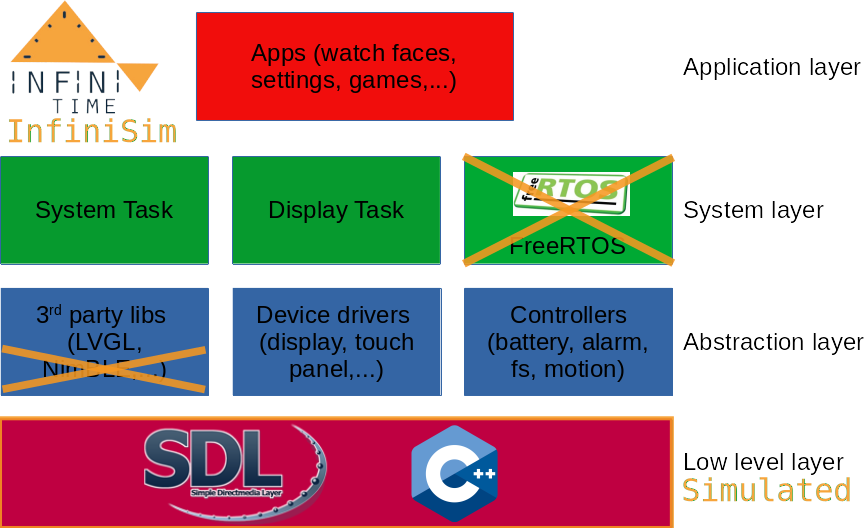
\includegraphics[width=\textwidth]{../architecture_infinisim}

  \small C++ Logo: Jeremy Kratz -
    \href{https://github.com/isocpp/logos}{https://github.com/isocpp/logos}\\
  \small SDL Logo: \href{https://www.libsdl.org}{https://www.libsdl.org}
\end{frame}

\section{Screens}
\subsection{Where to start?}
\begin{frame}{}
  \begin{itemize}
    \item Something easy
    \item little dependencies
  \end{itemize}
  \includegraphics[width=\textwidth]{../ponies_thinking}

  \small \href{http://awthredestim.blogspot.com/2012/04/my-little.html}{My Little Pony: Friendship is Magic. Season 2 "Ponyville Confidential"}
\end{frame}

\begin{frame}[fragile]{}

  Minimal Screen Constructor
  \begin{verbatim}
Screen(DisplayApp* app, LittleVgl& lvgl);
  \end{verbatim}

  Copy depedencies and comment out everything I haven't handled yet

  \begin{verbatim}
src/displayapp/DisplayApp.h
    -> sim/displayapp/DisplayApp.h
src/displayapp/DisplayApp.cpp
    -> sim/displayapp/DisplayApp.cpp
src/displayapp/LittleVGL.h
    -> sim/displayapp/LittleVGL.h
src/displayapp/LittleVGL.cpp
    -> sim/displayapp/LittleVGL.cpp
  \end{verbatim}
\end{frame}

\begin{frame}{}
  % convert rainboom.mp4 -coalesce rainboom.mp4 rainboom.png
  \includegraphics[width=\textwidth]{../rainboom-0}
\end{frame}

\subsection{2021-10-13 Paddle}
\begin{frame}{}
  \centering\includegraphics[height=0.8\paperheight]{../2021-10-13_Paddle.png}
\end{frame}

\subsection{2021-11-03 Paint, Fonts and Swipes}
\begin{frame}{}
  \centering
  \includegraphics[height=0.8\paperheight]{../2021-11-03_InfiniPaint_logo.png}

  Writes directly to framebuffer, headache to simulate
\end{frame}
\begin{frame}{}
  \centering
  \includegraphics[height=0.8\paperheight]{../2021-11-03_Paddle_with_fonts.png}

  Found the fonts! Now it looks like on the watch
\end{frame}
\begin{frame}{}
  \centering
  \includegraphics[height=0.8\paperheight]{../2021-11-03_Twos_first_sim.png}

  First swipes gestures implemented
\end{frame}


\subsection{2021-11-07 Metronome and the Motor}
\begin{frame}{}
  \centering\includegraphics[width=\textwidth]{../2021-11-07_metronome_and_motor_status.png}

  First external hardware simulated: MotorController
\end{frame}

\subsection{2021-11-15 BatteryInfo}
\begin{frame}{}
  \centering\includegraphics[height=0.8\paperheight]{../2021-11-15_BatteryInfo.png}

  Battery Empty??? Jokes on you! My PC has no battery!
\end{frame}

\subsection{2021-11-18 Found my Simulated Charger}
\begin{frame}{}
  \centering\includegraphics[width=\textwidth]{../2021-11-18_BatteryInfo_charging.png}

  Found my simulated charging cable
\end{frame}

\subsection{Screen switching, the hard(-coded) way}
\begin{frame}{}
  \centering\includegraphics[width=\textwidth]{../switching_screens_hard_coded}

  comment, uncomment, recompile, restart
\end{frame}

\subsection{Screen switching, by the key-press}
\begin{frame}{}
  \centering\includegraphics[width=\textwidth]{../switching_screens_function}

  hit key on keyboard, success!
\end{frame}

\subsection{2021-11-30 It's Time! Isn't it?}
\begin{frame}{}
  \centering\includegraphics[width=0.49\textwidth]{../2021-11-30_WatchFaceDigital}
  \centering\includegraphics[width=0.49\textwidth]{../2021-11-30_WatchFaceAnalog}
  %\centering\includegraphics[width=0.49\textwidth]{../2021-11-30_PineTimeStyle}
\end{frame}

\subsection{2021-12-02 It's Time! I knew it!}
\begin{frame}{}
  \centering\includegraphics[width=0.49\textwidth]{../2021-12-02_WatchFaceDigital_notified}
  \centering\includegraphics[width=0.49\textwidth]{../2021-12-02_WatchFaceAnalog_notified}
  %\centering\includegraphics[width=0.49\textwidth]{../2021-12-02_PineTimeStyle_notified}
\end{frame}

\subsection{2021-12-02 Time with PineTimeStyle and QuickSettings}
\begin{frame}{}
  \centering\includegraphics[width=0.49\textwidth]{../2021-12-02_PineTimeStyle_notified}
  \centering\includegraphics[width=0.49\textwidth]{../2021-12-02_QuickSettings}
\end{frame}

\subsection{2021-01-25 The real deal: Swiping! No more keys!}
\begin{frame}{}
  \centering\includegraphics[width=\textwidth]{../2022-01-25_swiping-0}

  \href{https://user-images.githubusercontent.com/9076163/151057090-66fa6b10-eb4f-4b62-88e6-f9f307a57e40.gif}{
    First swiping gif of InfiniSim\\
  \quad \small https://user-images.githubusercontent.com/9076163/151057090-66fa6b10-eb4f-4b62-88e6-f9f307a57e40.gif}
\end{frame}

\section{InfiniSim Project}

\subsection{2022-02-12 You've got mail!}
\begin{frame}{}

  \centering\includegraphics[width=0.9\textwidth]{../2022-02-12_jf002_matrix}

\end{frame}

\begin{frame}{}

  \centering\includegraphics[width=0.8\textwidth]{../pony_rainbow_omg_omg}

\end{frame}

\subsection{2022-02-17 Initial Commit}
\begin{frame}{}
  \centering\includegraphics[width=0.9\textwidth]{../2022-02-17_InfiniSim_initial_commit}
\end{frame}

\subsection{2022-02-20 a wild PinePhonePro appears}
\begin{frame}{}

  \centering\includegraphics[width=0.9\textwidth]{../2022-02-20_InfiniSim_on_PinePhonePro}

\end{frame}

\section{Links}
\subsection{The End}
\begin{frame}{}

  \href{https://user-images.githubusercontent.com/9076163/151057090-66fa6b10-eb4f-4b62-88e6-f9f307a57e40.gif}{
    First swiping gif of InfiniSim\\
  \quad \small https://user-images.githubusercontent.com/\\
  \quad\quad 9076163/151057090-66fa6b10-eb4f-4b62-88e6-f9f307a57e40.gif}

  \medskip
  \href{https://video.codingfield.com/videos/watch/f75c378e-bb0e-4b01-965a-64466c40ee36}{
    Video - InfiniSim on the PinephonePro\\
  \quad \small https://video.codingfield.com/videos/watch/\\
  \quad\quad f75c378e-bb0e-4b01-965a-64466c40ee36}

  \medskip
  \href{https://twitter.com/codingfield/status/1495505602746986502}{
    Twitter - InfiniSim on the PinephonePro\\
  \quad \small https://twitter.com/codingfield/status/1495505602746986502}

  \medskip
  \href{https://mastodon.codingfield.com/@JF/107832366241507784}{
    Mastodon - InfiniSim on the PinephonePro\\
  \quad \small https://mastodon.codingfield.com/@JF/107832366241507784}

  \medskip
  \href{https://github.com/InfiniTimeOrg/InfiniSim}{
    InfiniSim\\
  \quad \small https://github.com/InfiniTimeOrg/InfiniSim}

\end{frame}

\end{document}

